\section{Posets of graph rewriting events}

\subsection{From transition systems to posets}

\begin{definition}[Causal trace]
  \label{def:causal_trace}
  Let $\theta:M_0\overset{m_1,p_1}{\Rightarrow} M_1\overset{m_2,p_2}{\Rightarrow} M_2 \cdots \overset{m_n,p_n}{\Rightarrow} M_n$ be a trace.
  Two transitions $t_1$ and $t_2$ of $\theta$ are high res dependent in $\theta$, if $t_1<_{\theta} t_2$ can be derived by the following rules:
  \begin{align*}
    \frac{t_1 < t_2}{t_1 <_{\theta} t_2}\quad
    \frac{t_1\simeq t_1'<t_2'\simeq t_2}{t_1 <_{\theta} t_2}
  \end{align*}
  Two transitions $t_1$ and $t_2$ of $\theta$ are low res dependent in $\theta$, if $t_1\prec_{\theta} t_2$ can be derived by similar rules to the ones above. In a similar manner, we define when a transition $t_1$ inhibits a transition $t_2$ of $\theta$, denoted $t_1\dashv_{\theta} t_2$.
  %% \begin{align*}
  %%   \frac{t_1 \dashv t_2}{t_1 \dashv_{\theta} t_2}\quad
  %%   \frac{t_1\simeq t_1'\dashv t_2'\simeq t_2}{t_1 \dashv_{\theta} t_2}
  %% \end{align*}
  Define $\leq$ the transitive and reflexive closure of low res dependence. We say that $\theta$ is a \emph{causal trace} if it is directed w.r.t. $\leq$.
\end{definition}

\begin{definition}[Augmented poset]
  Let $s=(E,\cover,\prec,\dashv,\labl)$ be a set of events equipped with three binary relations on events $\cover$, $\prec$, $\dashv$ and a labelling function $\labl:E\to R$. We can retrive a poset from $s$, denoted $(E,\leq)$, where $\leq$ is the transitive and reflexive closure of $\prec$.
  %Let $s=(E, \leq,\dashv,\labl)$ be a set of events equipped with a partial order $\leq$, a binary relation on events $\dashv$ and a labelling function $\labl:E\to R$.
  We call $s$ an \emph{augmented poset}.
\end{definition}

\begin{definition}[The abstraction on a trace]
  \label{def:abstraction}
  Let us denote with $\Theta$ the set of causal traces.
  Define $\alpha:\Theta\to\mathcal{S}$ an \emph{abstraction} function that maps a trace into a poset as follows:
    \begin{itemize}
    \item given a transition $t:M\overset{m,p}{\Rightarrow} M'$ define the \emph{abstract event} $e$ associated to it
      $\alpha(t) = e_t$ such that $\labl(e) = p$.
    \item define an augmented poset from a trace $\alpha(\theta) = (E,\cover,\dashv,\labl)$ such that $\alpha$ is a bijection between transitions and abstract events and such that the sequential dependence and inhibition relations between transitions is preserved:
      \begin{align*}
        %\alpha(t_i:M_{i-1}\overset{m_{i},p_{i}}{\Rightarrow}M_i) = e_i \\
        e_i \cover e_j \iff t_i <_{\theta} t_j \text{ and } \alpha(t_i)=e_i, \alpha(t_j)=e_j\\
        e_i \prec e_j \iff t_i \prec_{\theta} t_j \text{ and } \alpha(t_i)=e_i, \alpha(t_j)=e_j\\
        e_i \dashv e_j \iff t_i \dashv_{\theta} t_j \text{ and } \alpha(t_i)=e_i, \alpha(t_j)=e_j.
      \end{align*}
    %% \item define a decorated poset from a trace $\alpha(\theta) = (E,\redl{+},\redl{-},\labl)$ such that $\alpha$ is a bijection between transitions and abstract events and such that the sequential dependence and inhibition relations between transitions is preserved:
    %%   \begin{align*}
    %%     %\alpha(t_i:M_{i-1}\overset{m_{i},p_{i}}{\Rightarrow}M_i) = e_i \\
    %%     e_i \redl{+}_O e_j \iff t_i <_{\theta} t_j, \labl(t_i) \redl{+}_O \labl(t_j)
    %%     \text{ and } \alpha(t_i)=e_i, \alpha(t_j)=e_j\\
    %%     e_i \redl{-}_O e_j \iff t_i \dashv_{\theta} t_j, \labl(t_i) \redl{-}_O \labl(t_j)
    %%     \text{ and } \alpha(t_i)=e_i, \alpha(t_j)=e_j.
    %%   \end{align*}
    \end{itemize}
  %\item
    Let $\Theta = \{\theta_1,\cdots,\theta_n\}$ be a set of causal traces.
    Define the set of augmented posets $\mathcal{S}$ obtained by abstraction on $\Theta$ as follows
    \[
    \alpha(\{\theta_1,\cdots,\theta_n\}) = (s_1,\cdots, s_k)\text{ with }k\leq n
    \]
    where for each augmented poset $s$ there exists at least one trace $\theta\in\Theta$ such that $\alpha(\theta) = s$.
  %\end{itemize}
\end{definition}

\begin{example}
  Let us consider the following rules and trace:
  \begin{align*}
    r_1:A \Rightarrow A, B\qquad r_2:A \Rightarrow C \qquad r_3: B,C \Rightarrow C\qquad
    A \overset{\id_A,r_1}{\Rightarrow} A, B \overset{\id_A,r_2}{\Rightarrow} B,C \overset{id_{B,C},r_3}{\Rightarrow}C.
  \end{align*}
  Let us denote $t_1$, $t_2$ and $t_3$ the three transitions. We have that $t_1<t_3$, $t_2<t_3$ and $t_2\dashv t_1$.
  Note that if the abstraction also "forgets" that $t_2\dashv t_1$ the concretisation retrieves the trace above and a second one where $t_1$ and $t_2$ are sequential independent:
  \begin{align*}
    A_1,A_2 \overset{\id_{A_1},r_1}{\Rightarrow} A_1,A_2,B \overset{\id_{A_2},r_2}{\Rightarrow} A_1,B,C \overset{id_{B,C},r_3}{\Rightarrow} A_1,C.
  \end{align*}
\end{example}

\begin{definition}[Decorated poset]
  \begin{enumerate}
  \item[] $~$
  \item Given a set of events $E$ and a labeling function $\labl$ on events, define a function $\decor:E\times E \to E\times E\times G$ that associates to a pair of events $(e,e')$ the following set
    \begin{align*}
      \decor_{+}(e,e') = \{(e,e',O) : O\text{ is a graph such that }\labl(e)\redl{+}_O \labl(e')\}\\
       \decor_{-}(e,e') = \{(e,e',O) : O\text{ is a graph such that }\labl(e)\redl{-}_O \labl(e')\}
    \end{align*}

  \item Let $s = (E,\cover,\dashv,\labl)$ be an augmented poset. A \emph{decorated} poset of $s$, denoted $s^{\star}$, is defined as follows
    \begin{align*}
      s^{\star} = (E,\redl{+},\redl{-},\labl), \text{ where }
      &e\redl{+}_O e' \iff (e,e',O)\in\decor_+(e,e')\text{ and }e\prec e'\\
      &e\redl{-}_O e' \iff (e,e',O)\in\decor_-(e,e')\text{ and }e\dashv e'\\
    \end{align*}
    We denote $\decor(s)$ the set of all decorated posets of $s$.
  \end{enumerate}
\end{definition}

Note that the notation $e\redl{+}_O e'$ is an overload of the notation $\labl(e)\redl{+}_O \labl(e')$. The first is defined on events using the abstraction function. The second, defined on rules, can be inferred from the rules itself.

\begin{definition}[Valid decorated poset]
  \label{def:constraints_poset}
  A decorated poset $s = (E,\redl{+},\redl{-},\labl)$ is \emph{valid} if the following hold:
  \begin{description}
  \item[directed]
    $s$ is directed w.r.t. the transitive and reflexive closure of $\redl{+}$;
  \item[events are not pairwise inhibiting]
    $\forall e_1,e_2\in s$, $e_1\redl{-}_s e_2\implies \neg(e_2 \redl{-}_{s'} e_1)$, for some $s$, $s'$;
  \item[events cannot inhibit their causes]
    $\forall e_1,e_2\in s$, $e_1\leq e_2\implies \neg(e_2 \redl{-}_{s} e_1)$, for some $s$;
  \item[constraints on decorating meets]
    $\forall e_1,e_2,e_3\in s$ such that $e_1\redl{+}_{s_1} e_3$ and $e_2\redl{+}_{O_2} e_3$, let $O_1\remb O\lemb O_2$ be the pullback of the span $O_1\lemb L_3 \remb O_2$.
If there is no $s$, $s'$ such that $e_1\redl{-}_s e_2$ and $e_2\redl{-}_{s'} e_1$ then there exists the morphisms $O\emb K_1$ and $O\emb K_2$ such that the diagram below commutes:
    \[
    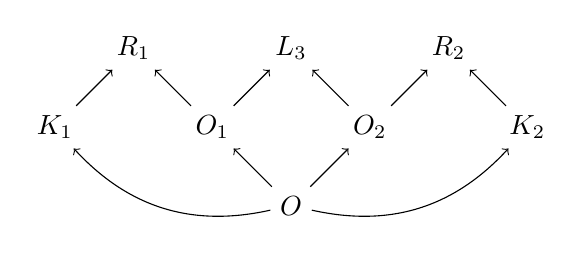
\begin{tikzpicture} %[scale=0.8]
      \node (o) at (0,-1) {\(O\)};
      \node (r3) at (0,1) {\(L_3\)};
      \node (o1) at (-1,0) {\(O_1\)};
      \node (o2) at (1,0) {\(O_2\)};
      \node (r1) at (-2,1) {\(R_1\)};
      \node (r2) at (2,1) {\(R_2\)};
      \node (k1) at (-3,0) {\(K_1\)};
      \node (k2) at (3,0) {\(K_2\)};
      \draw [->] (o) -- (o1);
      \draw [->] (o) -- (o2);
      \draw [->] (o1) -- (r3);
      \draw [->] (o2) -- (r3);
      \draw [->] (o1) -- (r1);
      \draw [->] (o2) -- (r2);
      \draw [->] (k1) -- (r1);
      \draw [->] (k2) -- (r2);
      \draw [->] (o) to [bend left] (k1);
      \draw [->] (o) to [bend right] (k2);
    \end{tikzpicture}
    \]
  \item[constraints on decorating joins]
    $\forall e_1,e_2,e_3\in s$ such that $e_3\redl{+}_{s_1} e_1$ and $e_3\redl{+}_{O_2} e_2$, let $O_1\remb O\lemb O_2$ be the pullback of the span $O_1\lemb L_3 \remb O_2$.
    If there is no $s$, $s'$ such that $e_1\redl{-}_s e_2$ and $e_2\redl{-}_{s'} e_1$ then there exists the morphisms $O\emb K_1$ and $O\emb K_2$ such that the diagram below commutes:
       \[
    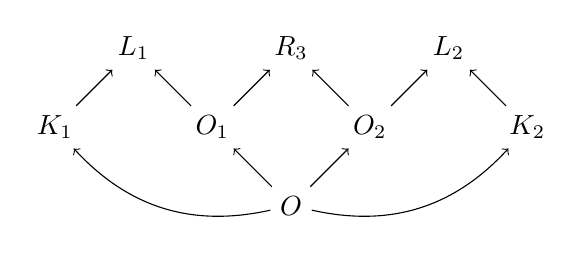
\begin{tikzpicture} %[scale=0.8]
      \node (o) at (0,-1) {\(O\)};
      \node (r3) at (0,1) {\(R_3\)};
      \node (o1) at (-1,0) {\(O_1\)};
      \node (o2) at (1,0) {\(O_2\)};
      \node (r1) at (-2,1) {\(L_1\)};
      \node (r2) at (2,1) {\(L_2\)};
      \node (k1) at (-3,0) {\(K_1\)};
      \node (k2) at (3,0) {\(K_2\)};
      \draw [->] (o) -- (o1);
      \draw [->] (o) -- (o2);
      \draw [->] (o1) -- (r3);
      \draw [->] (o2) -- (r3);
      \draw [->] (o1) -- (r1);
      \draw [->] (o2) -- (r2);
      \draw [->] (k1) -- (r1);
      \draw [->] (k2) -- (r2);
      \draw [->] (o) to [bend left] (k1);
      \draw [->] (o) to [bend right] (k2);
    \end{tikzpicture}
    \]
  \end{description}
  where $\labl(e_i)=r_i:L_i\remb K_i\lemb R_i$.
\end{definition}


We show in~\autoref{sec:valid_decor} that an abstraction from a causal trace to a decorated poset only produces valid decorations.


%% \begin{example} - for the cover relation
%%   Let us consider the following rules:
%%   \begin{align*}
%%     r_1:\varepsilon \Rightarrow A, B\qquad r_2:A \Rightarrow C \qquad r_3: B,C \Rightarrow C
%%   \end{align*}
%%   and the trace
%%   \begin{align*}
%%     \varepsilon \overset{\emptyset,r_1}{\Rightarrow} A, B \overset{\id_A,r_2}{\Rightarrow} B,C \overset{id_{B,C},r_3}{\Rightarrow}C.
%%   \end{align*}
%%   Let us denote $t_1$, $t_2$ and $t_3$ the three transitions. We have that $t_1<t_3$, $t_2<t_3$ and $t_1< t_2$. If we "forget" that $t_1< t_3$ (as both $t_1<t_2$ and $t_2<t_3$ hold), we retrieve the following trace:
%%   \begin{align*}
%%     B_1 \overset{\emptyset,r_1}{\Rightarrow} B_1,A,B_2 \overset{\id_{A},r_2}{\Rightarrow} B_1,A,B_2,C \overset{id_{B_1,C},r_3}{\Rightarrow} B_2,A_1,C.
%%   \end{align*}
%% \end{example}

\begin{example}
  If, in the following trace $\theta$, produced by the transitions $t_1;t_2;t_3$, we forget the decoration we obtain a poset with three events $e_1,e_2,e_3$ such that $e_1<e_3$ and $e_2<e_3$.
  \[
  \theta:\varepsilon \Rightarrow A \Rightarrow A,B\Rightarrow A,B,C\qquad t_1: \varepsilon \Rightarrow A\qquad t_2: \varepsilon\Rightarrow A,B\qquad t_2: A,B\Rightarrow A,B,C
  \]
  But we can come up with two decorations for such poset, where one of them leads to a invalid decorated poset:
  \begin{align*}
  \text{good decoration: }&e_1\redl{+}_A e_3\qquad e_2\redl{+}_B e_3\\
  \text{bad decoration: }&e_1\redl{+}_A e_3\qquad e_2\redl{+}_A e_3
  \end{align*}
\end{example}

\begin{mdframed}[backgroundcolor=blue!20]
to do: the other examples on decoration.
\end{mdframed}



\subsection{From posets to traces}

\begin{definition}[Refinement of an event in a trace]
  Let $E$ be a set of events and let $\theta$ be a trace. A refinement function is a bijection between events and transitions such that
  \[
  \mathtt{Ref}(e) = M\overset{m,\labl(e)}{\Rightarrow}N
  \]
  We say that $\mathtt{Ref}(e)$ is the refinement of $e$ in $\theta$ given a bijection $\mathtt{Ref}$.
\end{definition}

\begin{definition}[Concretisation of an augmented poset]
  \label{def:concret}
  Let $\underline s=(E,\cover,\prec,\dashv,\labl)$ be an augmented poset $s$.
  A \emph{concretisation} of $s$ is a triple $(s,\theta,\mathtt{Ref}:E\leftrightarrow\theta)$ such that $\mathtt{Ref}$ is a refinement function and such that
  \begin{align*}
    e_1\cover e_2 \iff& \mathtt{Ref}(e_1) <_{\theta}\mathtt{Ref}(e_2)\\
    e_1\prec e_2 \iff& \mathtt{Ref}(e_1) \prec_{\theta}\mathtt{Ref}(e_2)\\
    e_1\dashv e_2 \iff& \mathtt{Ref}(e_1) \dashv_{\theta}\mathtt{Ref}(e_2)
  \end{align*}
  Define $\gamma(s)$ to be the set of all concretisations of $s$:
  \begin{align*}
    \gamma(s) = \{\theta: (s,\theta,\mathtt{Ref})\text{ is a concretisation of }s\}.
  \end{align*}
\end{definition}

\begin{theorem}
  Let $\theta$ be a causal trace. Then $\theta\subseteq\gamma(\alpha(\theta))$.
\end{theorem}
\begin{proof}
  Suffices to show that for any causal trace $\theta$ there exists a refinement bijection between $\alpha(\theta)$ and $\theta$ that satisfies the constraints in~\autoref{def:concret}. It follows from~\autoref{def:abstraction}.
\end{proof}

%%%%%the algorithm%%%%%%%

\begin{definition}[Linear extensions of posets]
  A linear extension, denoted $\underline{s}$, of a poset $s=(E,\tleq)$ is any total order that extends the partial order $\tleq$. We denote $\linear(s)$ the set of all possible linear extensions of $s$. A linear extension of a augmented poset $s=(E,\cover,\prec,\dashv)$ is any total order such that
  \begin{align*}
    (E,\seq)\in\linear(s) \iff \forall e_1,e_2\in E, &e_1\leq e_2\implies e_1\seq e_2\\
    & e_1\dashv e_2\implies e_2\seq e_1.
  \end{align*}
\end{definition}


\subsection{Interpreting inhibition on posets}

\begin{definition}[Refinement based on negative influence]
  \label{def:ref_neg_infl}
  Let $s_1,s_2$ be two augmented posets and let $(s_1,\theta_1,\mathtt{Ref}_1)$ and $(s_2,\theta_2,\mathtt{Ref}_2)$ be two concretisations for $s_1$ and $s_2$ respectively.
  Define $\mathtt{Ref}(e_1\in s_1\redl{-} e_2\in s_2)$ as the set of graphs $M$ for which the diagram below commutes:
  \[
  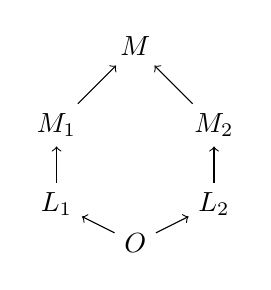
\begin{tikzpicture} %[scale=0.8]
    \node (o) at (0,-0.5) {\(O\)};
    \node (n) at (0,2) {\(M\)};
    \node (l1) at (-1,0) {\(L_1\)};
    \node (l2) at (1,0) {\(L_2\)};
    \node (n1) at (-1,1) {\(M_1\)};
    \node (n2) at (1,1) {\(M_2\)};
    \draw [->] (l1) -- (n1);
    \draw [->] (l2) -- (n2);
    \draw [->] (o) -- (l1);
    \draw [->] (o) -- (l2);
    \draw [->] (n1) -- (n);
    \draw [->] (n2) -- (n);
  \end{tikzpicture}
  \]
  where $\mathtt{Ref}_1(e_1) = M_1\Rightarrow N_1$, $\mathtt{Ref}_2(e_2) = M_2\Rightarrow N_2$, and $\labl(e_1)\redl{-}_s\labl(e_2)$, for some cospan $s:L_1\remb O\lemb L_2$
\end{definition}
